% !TEX root = ../TUCthesis.tex

%************************************************
\chapter{Background}\label{ch:Background}
%************************************************

A \ac{WSN} is a bunch of wireless devices connected together in a certain order to monitor physical or environmental conditions. Each of these devices is connected to one or several other sensors forming a network. Generally, every sensor node comprises of a radio transceiver (to send and receive messages), a microcontroller, sensors and a power source. The size of these devices can vary from the size of dust particle to the size of a notebook. They are constrained in memory, computational power, communication bandwidth and energy budget and are often deployed together in one of the several possible topologies including star, ring, tree or multi-hop mesh network. The propagation of data between the hops of the network can be routing or flooding. We can see a multi-hop mesh organisation of these nodes in figure \ref{fig:wsn-organisation}.

\par
In this figure, each of these devices have a sensor field in which they can communicate with the devices sharing a common sensor field space. The small circles in the figure \ref{fig:wsn-organisation} represent the \acp{SN} in multi-hop mesh network. In this topology, the data acquired by a \ac{SN} is routed to the sink with the help of the neighboring \acp{SN}. Finally when the data reaches the \ac{BS}, it is processed and further sent to an external network. These devices generally adhere to IEEE 802.15.4 Zigbee protocol (\cite{ieee:802.15.4}). This protocol is widely used for small low-powered digital radios and therefore find large number of application areas such as industrial Control and Monitoring, environmental and Health Monitoring, home Automation, entertainment and toys, security, location and asset tracking, emergency and disaster Response. Some of the features of this protocol include data rates of $250 kb/s (2.4 GHz)$ and $20/40 kb/s (868/915 MHz)$, $16$ channels in the $2.4 GHz$ ISM band, $10$ channels in the $915 MHz$ ISM band and one channel in the European $868 MHz$ band, carrier sense multiple access with a collision avoidance channel access, fully handshaked protocol for transfer reliability, extremely low duty-cycle $(< 10 ppm)$ capability, availability of beaconless operation and support for low latency devices.

\begin{figure}
    \centering
    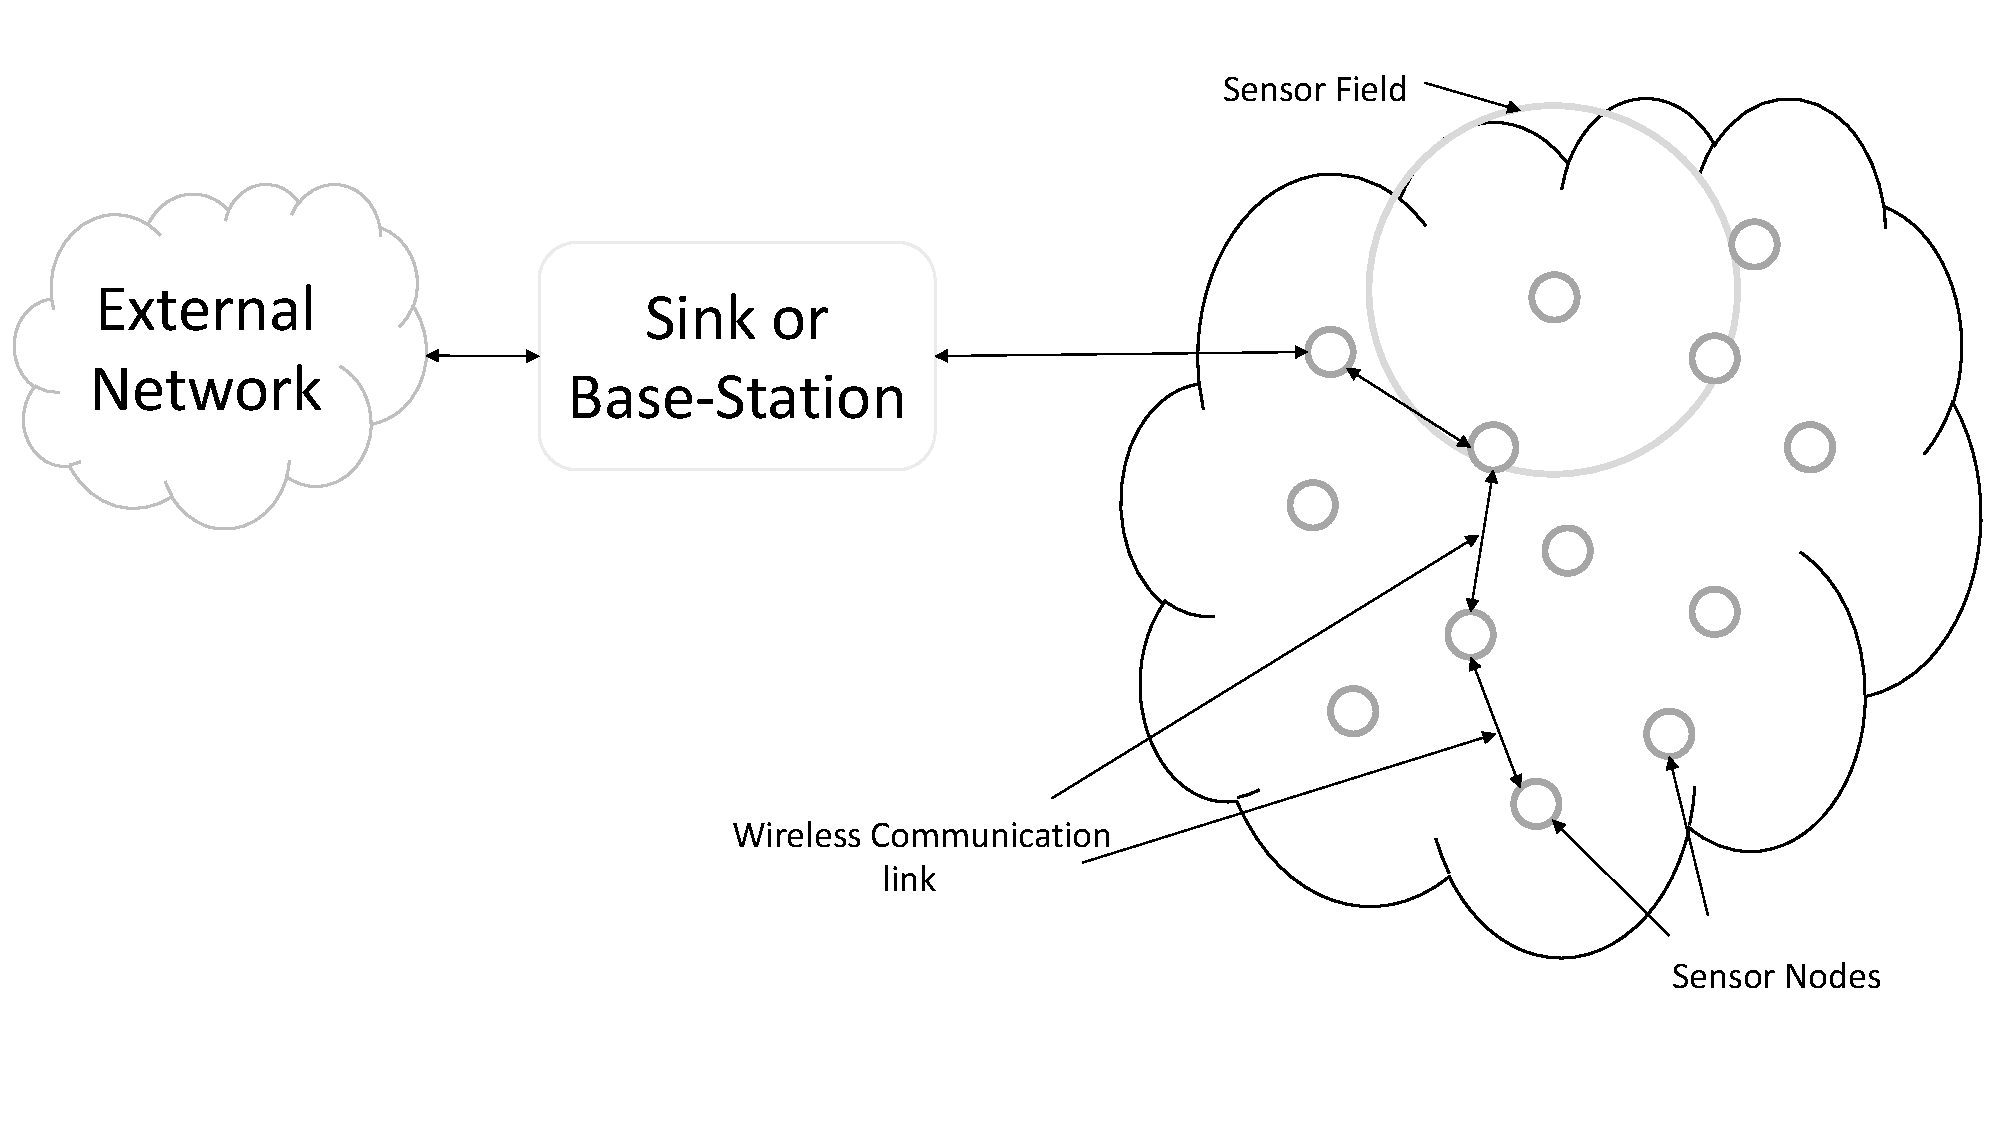
\includegraphics[width=1.0\textwidth]{gfx/WSNDiagram.pdf}
    \caption{\acp{WSN} Organisation}
    \label{fig:wsn-organisation}
\end{figure}


%************************************************
\section{Structure of Wireless Sensor Network}
%************************************************

The seven layer OSI model \cite{zimmermann1980osi}, is not suitable for implementation in low powered sensor devices. Therefore, in order to reduce the implementation complexity, the \ac{WSN} protocol stack is divided into five layers as shown in the figure \ref{fig:Wireless-Sensor-Network-Architecture}.

In this structure, each layer performs a set of tasks which is independent of other layers in the model. The physical layer deals with transferring a stream of bits over physical medium, signal detection and modulation, data encryption and connector cables compatibility with communication medium. The second layer, the data link layer provides services such as medium access control and error control, reliable data delivery, error detection and error correction. The third layer, the network layer is responsible for establishing communication paths between \acp{SN} and thereafter transmitting the packets along this path. The path selection phase depends on the one of the possible metrics: shortest path, energy efficiency, reliability and so on. The main tasks of this layer includes power conserving, partial memory, buffers, and self-organisation of \acp{SN} (because the \acp{SN} do no have universal ids). The protocols for routing layer can be separated into; flat routing and hierarchical routing or can also be separated into time driven, query-driven and event driven. The fourth layer, the transport layer provides transparent and reliable communications between end users. Two of the most widely used transport layer protocols are connection-oriented protocol, \ac{TCP} and connection-less protocol \ac{UDP}. \ac{TCP} provides reliable communication service and ensures guaranteed data delivery whereas \ac{UDP} provide an un-reliable service. In \ac{WSN} domain reliable loss recovery is more energy efficient than \ac{TCP} based communication. The final layer, the application layer is the mostly used layer for designing a\ac{WSN} application. It deals with the processing of sensed information, encryption, the formatting and storage of data and is also responsible for traffic management. It often uses information from other layers to detect if the application can meet the required resources.

\begin{figure}
    \centering
    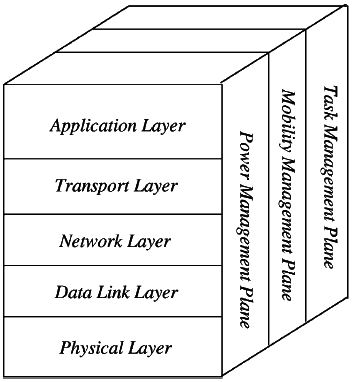
\includegraphics[width=1.0\textwidth,height=5cm,keepaspectratio]{Diagrams/Wireless-Sensor-Network-Architecture.png}
    \caption{\acp{WSN} Protocol Stack}
    \label{fig:Wireless-Sensor-Network-Architecture}
\end{figure}

\par

The three cross planes in the figure \ref{fig:Wireless-Sensor-Network-Architecture} are; power management plane, mobility management plane and task management plane. These layers help to manage the network and allow the \acp{SN} to work in conjunction with each other so that the overall efficiecy of a \ac{WSN} increases. 

%************************************************
\section{Application Areas}
%************************************************

Due to recent advancements in \acp{WSN}, it  are used in a large number of application scenarios. Some of them are listed below:

\begin{enumerate}
    \item Disaster relief operations: \acp{SN} monitor changes in environment (temperature, humidity and so on) and thus assist in disaster relief operations. They are also deployed to monitor water level in rivers to prevent flood consequences \cite{cayirci2007sendrom}.  
    
    \item Bio-diversity mapping: Observing wildlife \cite{juang2002energy}
    
    \item Intelligent buildings: Smart homes which can control the functioning of gadgets based on environmental conditions \cite{han2010smart}.
    
    \item Medicine and health care: Long-term monitoring of chronically ill patients \cite{pantelopoulos2010survey}.
    
    \item Agriculture: Monitoring soil and environment conditions to determine the amount of additives like fertilizers, water for better yield \cite{baggio2005wireless}.
\end{enumerate}

\section{nesC and TinyOS}{\label{section:nescTinyOS}}
%************************************************
This section will describe about the fundamentals of using nesC programming language (\cite{website:nesc}) in TinyOS. In the first subsection we will explain about the structure of a nesC program and in second part we will describe about the abstractions involved in sending and receiving messages using TinyOS. We will also talk about the data structures offered in TinyOS and finally we will describe the limitations of using TinyOS.   

    %************************************************
    \subsection*{nesC}
    %************************************************
    
    As an extension to C programming language, it defines the structure of TinyOS applications in components. The components are further modularized into interfaces, modules and configurations. Let us go through them one by one:
    
    \begin{enumerate}
        \item Interfaces:
        
        The notion of interface in nesC is similar to the concept of \textit{Interfaces} in Java or any other Object-oriented programming language. They define methods that can be implemented by a module. However, a major difference is: only events defined under interfaces must be implemented and commands can be called whenever required. For example Leds Interface provides these methods:
        
        \begin{lstlisting}
        
            interface Leds {
            
              // Turn on LED 0.
              async command void led0On();
            
              //Turn off LED 0.
              async command void led0Off();
            
              /**
               * Toggle LED 0; if it was off, turn it on, if was on, turn it off.
               * The color of this LED depends on the platform.
               */
            async command void led0Toggle();
            
            ...
            ...
        \end{lstlisting}
        
        Now to turn on the Leds on the Telosb, when required, we need to first use the interface called $Leds$ in our application by stating the following:
        
        \begin{lstlisting}{language = C}
            use interface{
                Leds;
            }
        \end{lstlisting}
        
        Then we have to call methods provided by Leds interface in our implementation. Leds interface provide methods to toggle(Leds.Led0toggle()) or turn on (Leds.Led0toggle()) the Leds on telosb board. Telosb led lights can be turned on by giving the command: 
        
        \begin{verbatim}
            call Leds.Led0On();
        \end{verbatim}
        
        We must note here that interfaces are prefixed with \textit{call} keyword. Also, there are parametrised interfaces to support multiple instances of same interface. The parameters for these multiple instances of interfaces can be small small integers.
        
        \item Modules and Configurations: Having discussed the interfaces concept, we will now look at the overall structure of a nesC program. A nesC program has two components: a file containing a module with its implementation, also known as \textit{Modules} and another file with configuration including the implementation, also called as \textit{Configurations}. Configurations, describe the wiring structure of components. In contrast to Configurations, Modules are implementations. Configurations connect the declarations  of  different  components,  while  modules  define  functions  and allocate state.
        
        Both modules and configurations can provide and use interfaces, but the main difference lie in their implementations. \textit{Configuration} implementations refer to how the interfaces used in modules are wired to the actual component that provides it. While \textit{Module} implementations are piece of executable codes that define how the provided interfaces should execute and return or how to use the interfaces to provide a new functionality. This will be clear in following example:
    
    \noindent\begin{minipage}{.40\textwidth}
    \begin{lstlisting}[title=Module,frame=tlrb]{Name}
    module BlinkC @safe()
    {
        uses interface Leds;
        uses interface Boot;
    }
    implementation
    {
        event void Boot.booted()
        {
            call Leds.led0Toggle();
        }
    }
    \end{lstlisting}
    \end{minipage}\hfill
    \begin{minipage}{.40\textwidth}
    \begin{lstlisting}[title=Configuration,frame=tlrb]{Name}
    configuration BlinkAppC
    {
    }
    implementation
    {
      components BlinkC, LedsC;
      BlinkC.Leds -> LedsC;
    }
    \end{lstlisting}
    \end{minipage}
    
    \end{enumerate}
    
    \par
    
    In the above code, the module section uses interface Leds and the implementation section calls \textit{Leds.led0Toggle()} to turn on the Leds on Telosb. Now, in the configuration section we need to instantiate LedsC component and further wire it to Leds interface used in module section so that the TinyOS points to the actual implementation of Leds, provided by LedsC component.

    %************************************************
    \subsection*{TinyOS}
    %************************************************
    
    TinyOS (\cite{website:TINYOS}) is the de facto standard in the field of \acp{WSN}. It provides network protocols, device driver for different sensor platforms, data capturing tools, single-hop networking, ad-hoc routing, timers and many other features, which can be easily used, with suitable modifications, for different application domains. It follows event-driven model which helps to run concurrent applications using small amount of memory. TinyOS uses Event driven models because they are faster than stack threaded design. This is because of two main reasons: 1. They do not require in-advance memory reservation to save execution context. 2. Hardware, is always split-phase rather than blocking. Because of non-blocking operations they perform the operations rapidly. In idle state, it goes in sleep state to save energy.
    
    \par
    A \ac{FIFO} based TinyOS scheduler schedules operations of components. This is also power efficient because the device can go in low power state when the queue is empty. Components are a collection of \textit{Command Handlers}, \textit{Event Handlers} and \textit{Tasks}. They contain the declarations of commands and events which are provided by the interface it uses or provides. After the declaration in Modules section, the interfaces in an application can be wired to the components which actually implements them. Let us look at these three components one by one:
    
    \begin{enumerate}
        \item Commands: Commands are non-blocking requests made to low-level components and therefore must return with the exit status whether it was successful or not. Commands can also schedule tasks for later execution. This will involve event handlers which can in turn execute other low level commands.
        
        \item Events:  In an embedded system application, we primarily focus on  handling events. In general, events are generated or triggered in response to some action that has been initiated by commands. Interfaces contain commands and events, and therefore when we use an interface, we must implement all the events, so that appropriate actions are defined when events are fired.
        
        \item Tasks: Tasks enable components to perform general-purpose "background" processing in an application. They are  non preemptive. This  means  that  only  one  task  runs  at any time, and TinyOS does not interrupt one task to run another. Once a task starts running, no other task runs until it completes. This means that  tasks  run  atomically  with  respect  to  one  another. This  has  the nice  property  that we  don’t  need  to  worry  about  tasks  interfering with one another and corrupting each other’s data. However, it also means that tasks should usually be reasonably short. If a component has a very long computation to do, it should break it up into multiple tasks. A task can post itself.
    \end{enumerate}
    
    \par
    To understand these components, we will consider the structure of AMSenderC component:
    
    \begin{verbatim}
        provides {
            interface AMSend;
            interface Packet;
            interface AMPacket;
            interface PacketAcknowledgements as Acks;
        }
    \end{verbatim}
    
    In the above example, if \textit{AMSend} interface is wired to \textit{AMSenderC} then it will be called as implemented in \textit{AMSenderC} component. Now, if we invoke \textit{AMSend.send()} method (provided by \textit{AMSend} interface) with a network packet (which is of type nx\_uint8\_t or nx\-uint16\_t) then it will schedule a task to send the packet which in turn will invoke an event handler \textit{AMSend.SendDone()} to acknowledge, if the sending operation was successful or not. Other aspects related to networking design will be covered further in \ref{subsec:network-architecture}
    
    \par
    There are following limitations in TinyOS:
    
    \begin{enumerate}
        \item Dynamic memory allocation is not allowed. This prevents run time memory allocation failures and memory fragmentation.
        
        \item Function pointers are also not allowed because TinyOS needs to know the complete execution graph of the program in advance.
    \end{enumerate}
    
    %************************************************
    \subsection*{TinyOS Networking Architecture}\label{subsec:network-architecture}
    %************************************************
    
    The maximum size of a TinyOS packet is 128 bytes including its headers and \ac{CRC}, which also matches the 802.15.4 specifications. An increase in packet size can lead to unpredicted errors in TinyOS. The core of communication abstraction comes from Active Messages (AM), a single-hop unreliable packet. They have a destination address and provide synchronous acknowledgement. The interfaces to send and receive messages in TinyOS are listed below:
    
    \begin{itemize}
        \item AMSend: This interface is used to send a message by calling the AMSend.Send command (provided by AMSend interface). On completion of successful or unsuccessful sending SendDone event is signalled. In general \ac{WSN} application development scenario, we also using this event as an indicator to send the next packet. 
        
        \item AMReceive: On reception of a message sent via AMSend interface, AMReceive.receive event of the corresponding AMSender id is signalled.
        
        \item AMSnoopingReceiver: This interface signals event AMSnoopingReceiver.receieve even when the packet is not addressed to a particular \ac{SN}. This allows us to snoop packets in the device communication range.
    \end{itemize}
    
    To send data, we need to instantiate a member of AMSend with an am\_id\_t type, which is a small integer, and further wire it to AMSend interface. We then need to call AMSend.send() method from the module implementation, which will trigger sending of \ac{AM} packet. The packet can either be sent to all the sensor nodes which is done by broadcasting at AM\_BROADCAST\_ADDR (a constant defined as 0xFFFF and is reserved in TinyOS for broadcasting purposes) or to a specified TOS\_NODE\_ID (every \ac{SN} has a specific address which can be obtained by calling TOS\_NODE\_ID constant).
    
    \par
    After a \ac{SN} receives an \ac{AM}, it calls events that are responsible to receive the messages of the defined \textit{am\_id\_t} type of Receive Component. This concept of multiple instances of same Component, gives us the flexibility to have multiple instances of Receivers (abstracted as \textit{AMReceiverC}). With multiple \ac{AM} ids of AMReceiverC, the device will only call the event associated with the matching receiver id. This concept is predominantly used in TinyOS to distinguish messages of different types and we will also use this in implementation of the concept \textit{heterogeneity} to distinguish one hop and two hop messages received. 
    
% This section describes how \ac{PC} advertises it's availability, \acp{SN} discovers the \ac{PC} and finally how data transfer takes place.

%************************************************
\section{Route Finding and Selection}    
%************************************************

Route discovery, route selection and route representation are key requirements for a wireless multi-hop routing problem. Therefore, it becomes quite important to decide appropriate protocols for finding a solution to multi-hop routing scenarios. We will cover the fundamentals to find a solution to the multi-hop routing problem by sequentially enumerating through the mentioned phases, as shown in the figure \ref{fig:RouteFinding}:

\begin{figure}[h]
    \centering
	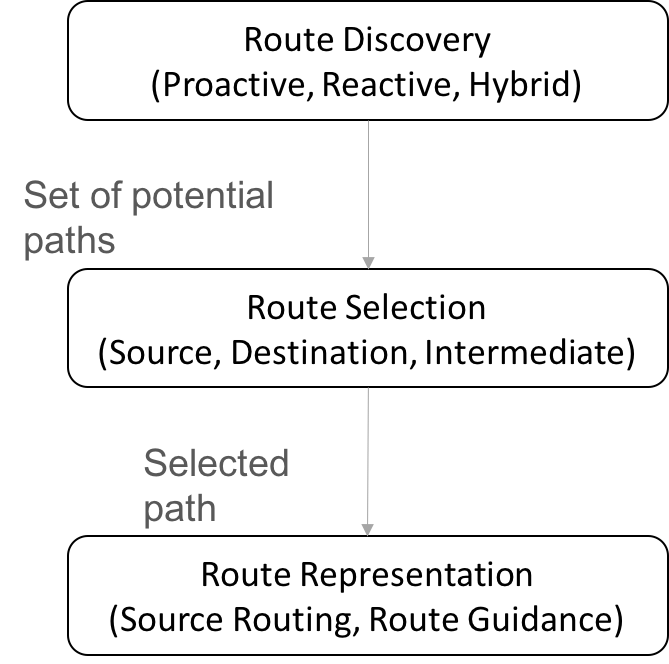
\includegraphics[height =5cm, keepaspectraio]{gfx/RouteFinding.png}
	\caption{Route Finding Phases}
	\label{fig:RouteFinding}
\end{figure}

\begin{enumerate}

    \item \label{enumerate:RouteDiscovery} Route Discovery: Three ways exist to find a route from source to destination:

    \begin{enumerate}
    
    	\item Proactive: Protocols like \ac{DVR} (\cite{RFC1058}) and \ac{OLSR} (\cite{RFC3626}) use pro-active techniques to find a route to the destination. They maintain routing tables to store information about how to reach the destination. Although this technique is quite good for high traffic but it has huge memory requirement to store tables for the entire network.
    	
    	\item Reactive: Protocols in this category, e.g. \ac{AODV} (\cite{RFC3561}) and \ac{DSR} (\cite{RFC4728}), perform on-demand  route discovery by sending a \ac{RREQ}, containing the desired destination address for data sending, to neighbors and receive a \ac{RREP} from the destination. Route discovery can be done in two pays: Firstly, doing it on fly. Under this technique route is searched whenever required. Secondly, it can be done hop-by-hop. In this technique each \ac{SN} decides the next suitable neighbor to forward the packet. \acp{SN} accomplish this task by exchanging periodic routing updates through beacons containing necessary information for neighborhood discovery.
    		
    	\item Hybrid: Protocols combining feature from both, proactive and reactive protocols.

    \end{enumerate}

    \item \label{enumerate:RouteSelection} Route Selection:
    
    For proactive protocols, route discovery phase is sufficient for route selection. Periodically updated routing tables provide the intended nodes with the information about how to reach destination nodes. However, this is not the case with reactive protocols. The selection phase can be handled by either of the three terminals: source, destination or the intermediate nodes.
    
    \par	
    The decision to make source or destination based route selection can depend on the application requirements. Hop count, end-to-end delay/jitter, interference level, packet loss rate, link residual capacity, load balancing and so on can be among the several possible metrics to select the net hop route. In general, number of hop counts to destination is often the preferred metric as it is easy to compute and also it provides us the shortest path to destination. For intermediate nodes, the route selection is done by every node on way to discover the best next hop. 
    
    \item Route Representation:
    
    Two approaches exist to achieve route representation: Either storing the exact route via routing tables/source routing or provide a route guidance. To implement the source routing approach, we need to include the exact route from the source to destination in the \ac{RREP} packet header. The sender then forwards the packet to the next recipient specified in the packet header. This process continues until the packet reaches the destination. In contrast to source routing, the route guidance method involves intermediate nodes to find the best next hop.
    
    In order to make the routing more efficient and to save energy by avoiding route re-computation to destination every now and then in heterogeneity, we will implement the idea of source routing in data transmission phase. In this mechanism we will let the sender know about the exact route to destination via which the data transmission phase should take place. This is discussed in more detail in chapter \ref{ch:Implementation}.
    
\end{enumerate}

%************************************************
\section{Data Collection}
%************************************************

Data collection is primarily used to collect sensor data captured by different \acp{SN} in a \ac{WSN}. The nodes collect information from their surroundings and forward this information to \ac{BS}. Data collected from deployed sensors can be further evaluated or analysed at the sink node or \ac{BS}. The fundamental idea is: generation of data at multiple nodes and collection at one node (called Root node or \ac{BS}). This pattern of flow of data also appears to be converging at one point. Efficient collection and reliable sending is a major challenge in the converging flow of the data. This requires quick adaptation to changes in the network without frequent beacon exchanges (because these exchanges consume considerable amount of energy). \ac{CTP} authors (\cite{TEP:119}) have claimed to solve the issues like reliability, robustness and high data delivery ratios.

\par
Most trivial way to realise this form of data collection is via tree establishment by following the below mentioned points:

\begin{itemize}
    \item Root nodes advertise themselves with hop count value 0 to the neighbors.
    \item Other \acp{SN} collect information like hop distance, node id and more from their neighborhood.
    \item Each \ac{SN} selects one of its neighbor as parent based on certain metrics (for examples refer to \ref{enum:linkqualitymeasures}).
    \item The parent nodes handle and forward the packets received from their children.
\end{itemize}

However there are following issues which also need to be taken care while establishing a tree.

\begin{itemize}
    \item Uni-directional links: A \ac{SN} determines the closest parent as the one which can only send packets but can not receive them.
    \item If a node accidentally receives one beacon from a far away node
    \item Mobile nodes: Node selected as parent is not in range because of it's mobile nature
\end{itemize}

Therefore, while selecting a parent we also include parameters to estimate link quality. Some of the ways to measure link quality are mentioned below:

\begin{enumerate}\label{enum:linkqualitymeasures}
    \item \ac{PRR}: Send a predefined number of packets and measure what fraction of these are received at regular intervals.
    
    \item \ac{RSSI}: Analyze received packets with regard to their signal strength (serving as an indicator for the node distance).

    
    \item \ac{LQI}: Correlation between bits in the \ac{SFD} to indicate potential channel issues (reflection, scattering, etc).

    \item \ac{ETX}: Estimate how many re-transmissions are needed on average when using a particular link.
\end{enumerate}

	
	%************************************************
	\subsection{Collection Tree Protocol}
	%************************************************
	
	\ac{CTP} is a \ac{DVR} protocol. \ac{DVR} is based on the idea of manipulating the vector distances to other \acp{SN} in the \ac{WSN}. Under this routing methodology, each \ac{SN} maintains a routing table consisting of following two information to reach each of the possible final destination \acp{SN}. 
	
	\begin{enumerate}
	    \item next node: Direction in which packet should be forwarded
	    \item cost: Hop counts from the destination
	\end{enumerate}
	
	Every entry in the next node column of the routing table must be an adjacent \ac{SN}, so that the intended sender can directly forward it's packets to this adjacent member. The table is maintained by periodic exchange of the vector consisting of the adjacent node routing table's cost column. Every \acp{SN} updates it's cost column by keeping the minimum of cost value it knows previously and the recently arrived cost vector. To avoid loops in the routing protocol, \ac{CTP} uses datapath validation technique. This technique gets rid of the routing loops by triggering routing updates when it encounters a data packet to be forwarded has lower \ac{ETX} value than it's current \ac{ETX} value or vice-versa or the \ac{ETX} value of a node drops significantly (in \ac{CTP} this threshold is 1.5). \ac{CTP} also uses adaptive beaconing mechanism to minimise power consumption and update stale information. The periodic timer to update stale information goes on increasing exponentially but the timer is reset as soon as the route update request is received. 
	
	\subsection{Implementation}
	
	In \ac{CTP}, \ac{ETX} metric is used to establish a tree topology for data collection. Every node broadcasts beacons indicating its \ac{ETX} to the sink. Broadcast intervals are exponentially increasing (up to 512 seconds), in static network conditions. Further, nodes select their parent based on the \ac{ETX} metric. Nodes compute their \ac{ETX} using the formula: 

    \[ \ac{ETX}_{ToSink} = \ac{ETX}_{Parent} + \ac{ETX}_{Node-ParentLink} \] 

    In this protocol parent can also be updated during run time when link with better \ac{ETX} becomes available. A \ac{SN} participating in \ac{CTP} collection, sends its data as uni-cast messages with link-layer acknowledgments enabled. TinyOS developers have included \ac{CTP} implementation in their operating system libraries. This can be found at \cite{tinyOS:ctpImplementation}. In the following section we will describe the main role taken by the software components of \ac{CTP} framework as shown in figure \ref{fig:CTPFramework}.
	
	\begin{center}
    \begin{figure}[h]
    	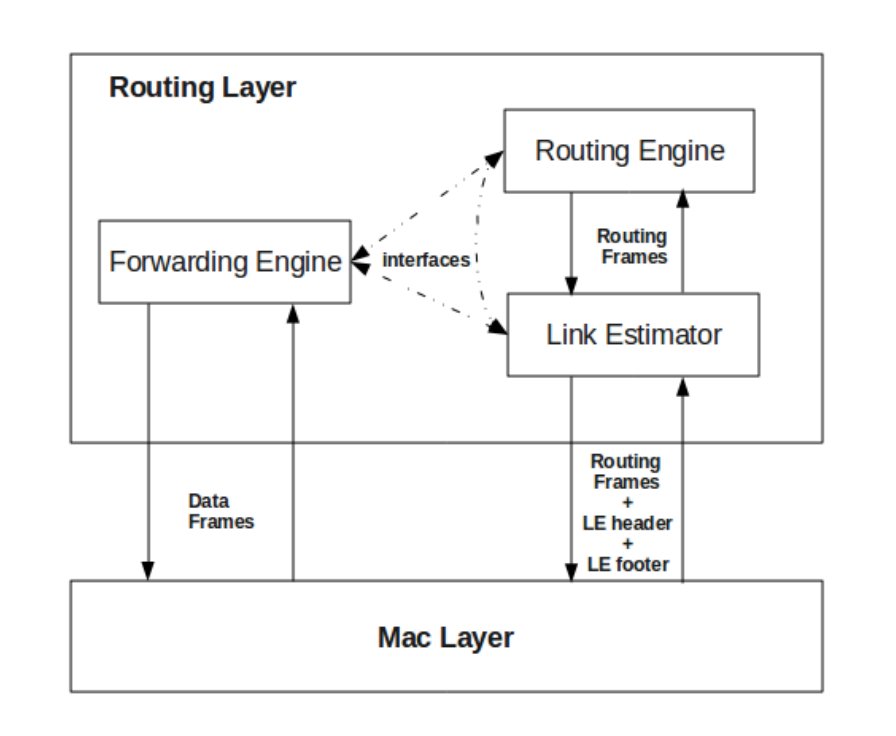
\includegraphics[height=10cm]{gfx/MessageFlowandmodulesInteractions.png}
    	\caption{Message flow and modules interactions, from \cite{colesanti2010performance}}
    	\label{fig:CTPFramework}
    \end{figure}
    \end{center}
	
    \begin{enumerate}
        
        \item Link estimation: This component provides the \ac{ETX} information for one hop communication between two \acp{SN}. This value is updated based on the adaptive beaconing strategy as mentioned in the above section. It also combines information from physical, data link, and network layers to provide accurate link quality estimates. For every 5 transmissions by the \ac{ETX} estimator, it produces an \ac{ETX} value of 6, if the number of successful transmissions is 0. The implementation for this module can be found in \cite{ctp:linkEstimation}.
        
        \item CtpRoutingEngineP: This component provides methods to select the next hop for data transmission based on the \ac{ETX} values obtained from Link Estimator. It also stores the minimum cost route to the root node. A root node advertises it's \ac{ETX} as zero and the \ac{ETX} of a \ac{SN} is calculated by adding the \ac{ETX} of it's parent node plus the \ac{ETX} of the link to it's parent node. 
        
        \ac{CTP} beacons are sent at specific intervals determined by Trickle algorithm. The algorithm allows to gradually reduce the beacon sending rate which further helps in saving energy and bandwidth. However, data path validations can reset this interval to make the \acp{SN} react to topological and environmental changes quickly.
    
        
        \item CtpForwardingEngineP: It is responsible for forwarding the packets received from child nodes as well as the data generated by the \ac{SN} itself. It also attempts retransmissions when necessary (in worst case up to 32 times). It also informs about the routing inconsistencies like routing loops to routing engine. 
        
    \end{enumerate}
    
    
	%************************************************
	\subsection*{CTP for Heterogeneity}
	%************************************************
    
    \par
    We have re-used existing metrics provided by \ac{CTP} for finding solution to best next hop discovery. This can be done by tweaking the routing engine component in \ac{CTP} (which establishes a collection tree to collect data at sink). Moreover, the information provided by \ac{CTP} is a reliable solution to find neighbors and estimate routes because the protocol considers information from link layer and routing layer to estimate the link quality. We will discuss in detail about the modifications and usage of \ac{CTP} in heterogeneity in chapter \ref{ch:Implementation}.